\documentclass[utf8x, 14pt, bold, times]{G7-32} % Стиль (по умолчанию будет 14pt)

\sloppy

% Настройки стиля ГОСТ 7-32
% Для начала определяем, хотим мы или нет, чтобы рисунки и таблицы нумеровались в пределах раздела, или нам нужна сквозная нумерация.
%\EqInChapter % формулы будут нумероваться в пределах раздела
%\TableInChapter % таблицы будут нумероваться в пределах раздела
%\PicInChapter % рисунки будут нумероваться в пределах раздела

% Добавляем гипертекстовое оглавление в PDF
\usepackage[
bookmarks=true, colorlinks=true, unicode=true,
urlcolor=black,linkcolor=black, anchorcolor=black,
citecolor=black, menucolor=black, filecolor=black,
]{hyperref}

\AfterHyperrefFix

% полезный пакет для микротипографии, увы под xelatex мало чего умеет,
% но под pdflatex хорошо улучшает читаемость
\usepackage{microtype}

% Тире могут быть невидимы в Adobe Reader
\ifInvisibleDashes
\MakeDashesBold
\fi

\usepackage{graphicx}   % Пакет для включения рисунков

% С такими оно полями оно работает по-умолчанию:
% \RequirePackage[left=20mm,right=10mm,top=20mm,bottom=20mm,headsep=0pt,includefoot]{geometry}
% Если вас тошнит от поля в 10мм --- увеличивайте до 20-ти, ну и про переплёт не забывайте:

\geometry{right=10mm}
\geometry{left=30mm}
\geometry{top=20mm}
\geometry{bottom=20mm}
% считать от нижней границы текста
\geometry{ignorefoot}


% Пакет Tikz
\usepackage{tikz}
\usetikzlibrary{arrows,positioning,shadows}

% Произвольная нумерация списков.
\usepackage{enumerate}

% ячейки в несколько строчек
\usepackage{multirow}

% itemize внутри tabular
\usepackage{array}

\usepackage{blindtext}

% Центрирование подписей к плавающим окружениям
%\usepackage[justification=centering]{caption}

\usepackage{newfloat}
\DeclareFloatingEnvironment[
placement={!ht},
name=Equation
]{eqndescNoIndent}
\edef\fixEqndesc{\noexpand\setlength{\noexpand\parindent}{\the\parindent}\noexpand\setlength{\noexpand\parskip}{\the\parskip}}
\newenvironment{eqndesc}[1][!ht]{%
    \begin{eqndescNoIndent}[#1]%
\fixEqndesc%
}
{\end{eqndescNoIndent}}

% Располагает все картинки (floats) до начала
% следующего раздела
\usepackage[section]{placeins}

% Двойная горизонтальная линия у таблиц
\usepackage{hhline}
% Расстояние между линиями
\setlength\doublerulesep{.5pt}

% Настройки листингов.
\usepackage{local-minted}

\usepackage{amsmath}
\makeatletter
\let\save@mathaccent\mathaccent
\newcommand*\if@single[3]{%
  \setbox0\hbox{${\mathaccent"0362{#1}}^H$}%
  \setbox2\hbox{${\mathaccent"0362{\kern0pt#1}}^H$}%
  \ifdim\ht0=\ht2 #3\else #2\fi
  }
%The bar will be moved to the right by a half of \macc@kerna, which is computed by amsmath:
\newcommand*\rel@kern[1]{\kern#1\dimexpr\macc@kerna}
%If there's a superscript following the bar, then no negative kern may follow the bar;
%an additional {} makes sure that the superscript is high enough in this case:
\newcommand*\widebar[1]{\@ifnextchar^{{\wide@bar{#1}{0}}}{\wide@bar{#1}{1}}}
%Use a separate algorithm for single symbols:
\newcommand*\wide@bar[2]{\if@single{#1}{\wide@bar@{#1}{#2}{1}}{\wide@bar@{#1}{#2}{2}}}
\newcommand*\wide@bar@[3]{%
  \begingroup
  \def\mathaccent##1##2{%
%Enable nesting of accents:
    \let\mathaccent\save@mathaccent
%If there's more than a single symbol, use the first character instead (see below):
    \if#32 \let\macc@nucleus\first@char \fi
%Determine the italic correction:
    \setbox\z@\hbox{$\macc@style{\macc@nucleus}_{}$}%
    \setbox\tw@\hbox{$\macc@style{\macc@nucleus}{}_{}$}%
    \dimen@\wd\tw@
    \advance\dimen@-\wd\z@
%Now \dimen@ is the italic correction of the symbol.
    \divide\dimen@ 3
    \@tempdima\wd\tw@
    \advance\@tempdima-\scriptspace
%Now \@tempdima is the width of the symbol.
    \divide\@tempdima 10
    \advance\dimen@-\@tempdima
%Now \dimen@ = (italic correction / 3) - (Breite / 10)
    \ifdim\dimen@>\z@ \dimen@0pt\fi
%The bar will be shortened in the case \dimen@<0 !
    \rel@kern{0.6}\kern-\dimen@
    \if#31
      \overline{\rel@kern{-0.6}\kern\dimen@\macc@nucleus\rel@kern{0.4}\kern\dimen@}%
      \advance\dimen@0.4\dimexpr\macc@kerna
%Place the combined final kern (-\dimen@) if it is >0 or if a superscript follows:
      \let\final@kern#2%
      \ifdim\dimen@<\z@ \let\final@kern1\fi
      \if\final@kern1 \kern-\dimen@\fi
    \else
      \overline{\rel@kern{-0.6}\kern\dimen@#1}%
    \fi
  }%
  \macc@depth\@ne
  \let\math@bgroup\@empty \let\math@egroup\macc@set@skewchar
  \mathsurround\z@ \frozen@everymath{\mathgroup\macc@group\relax}%
  \macc@set@skewchar\relax
  \let\mathaccentV\macc@nested@a
%The following initialises \macc@kerna and calls \mathaccent:
  \if#31
    \macc@nested@a\relax111{#1}%
  \else
%If the argument consists of more than one symbol, and if the first token is
%a letter, use that letter for the computations:
    \def\gobble@till@marker##1\endmarker{}%
    \futurelet\first@char\gobble@till@marker#1\endmarker
    \ifcat\noexpand\first@char A\else
      \def\first@char{}%
    \fi
    \macc@nested@a\relax111{\first@char}%
  \fi
  \endgroup
}
\makeatother

% 8 Листинги

\usepackage{listings}

% Значения по умолчанию
\lstset{
  basicstyle=\footnotesize,
  breakatwhitespace=true,% разрыв строк только на whitespacce
  breaklines=true,       % переносить длинные строки
%   captionpos=b,          % подписи снизу -- вроде не надо
  inputencoding=koi8-r,
  numbers=left,          % нумерация слева
  numberstyle=\footnotesize,
  showspaces=false,      % показывать пробелы подчеркиваниями -- идиотизм 70-х годов
  showstringspaces=false,
  showtabs=false,        % и табы тоже
  stepnumber=1,
  tabsize=4,              % кому нужны табы по 8 символов?
  frame=single
}

% Стиль для псевдокода: строчки обычно короткие, поэтому размер шрифта побольше
\lstdefinestyle{pseudocode}{
  basicstyle=\small,
  keywordstyle=\color{black}\bfseries,%\underbar,
  language=Pseudocode,
  numberstyle=\footnotesize,
  commentstyle=\footnotesize\it
}

% Стиль для обычного кода: маленький шрифт
\lstdefinestyle{realcode}{
  basicstyle=\scriptsize,
  numberstyle=\footnotesize
}

% Стиль для коротких кусков обычного кода: средний шрифт
\lstdefinestyle{simplecode}{
  basicstyle=\footnotesize,
  numberstyle=\footnotesize
}

% Стиль для BNF
\lstdefinestyle{grammar}{
  basicstyle=\footnotesize,
  numberstyle=\footnotesize,
  stringstyle=\bfseries\ttfamily,
  language=BNF
}

% Определим свой язык для написания псевдокодов на основе Python
\lstdefinelanguage[]{Pseudocode}[]{}{
  morekeywords={begin, end, if, else, while, for, step, to, downto, byte, word, and},% ключевые слова добавлять сюда
  morecomment=[s]{\{}{\}},% комменты {а-ля Pascal} смотрятся нагляднее
  literate=% а сюда добавлять операторы, которые хотите отображать как мат. символы
    {->}{\ensuremath{$\rightarrow$}~}2%
    {<-}{\ensuremath{$\leftarrow$}~}2%
    {:=}{\ensuremath{$\leftarrow$}~}2%
    {<--}{\ensuremath{$\Longleftarrow$}~}2%
}[keywords,comments]

% Свой язык для задания грамматик в BNF
\lstdefinelanguage[]{BNF}[]{}{
  morekeywords={},
  morecomment=[s]{@}{@},
  morestring=[b]",%
  literate=%
    {->}{\ensuremath{$\rightarrow$}~}2%
    {*}{\ensuremath{$^*$}~}2%
    {+}{\ensuremath{$^+$}~}2%
    {|}{\ensuremath{$|$}~}2%
}[keywords,comments,strings]

% Подписи к листингам на русском языке.
\renewcommand\lstlistingname{Листинг}
\renewcommand\lstlistlistingname{Листинги}


\begin{document}

\frontmatter % выключает нумерацию ВСЕГО; здесь начинаются ненумерованные главы: реферат, введение, глоссарий, сокращения и прочее.

\newcommand{\university}{
    Федеральное~государственное~автономное \\
    образовательное~учреждение \\
    высшего образования \\
    <<СИБИРСКИЙ~ФЕДЕРАЛЬНЫЙ~УНИВЕРСИТЕТ>>}
\newcommand{\faculty}{Институт~космических~и~информационных~технологий}
\newcommand{\department}{Кафедра~прикладной~математики~и~компьютерной~безопасности}
\newcommand{\city}{Красноярск}
\newcommand{\docname}{ОТЧЕТ~ПО~ЛАБОРАТОРНОЙ~РАБОТЕ}
\newcommand{\num}{~№3}
\newcommand{\topic}{Современные симметричные шифры. AES-128/AES-256.}
\newcommand{\variant}{Вариант~№~1}
\newcommand{\tutorname}{Ю.~В.~Потылицина}
\newcommand{\studentname}{С.~А.~Абрамов}
\newcommand{\group}{КИ20-08Б}
\newcommand{\gradebook}{032049480}

\renewcommand*{\maketitle}{
\begin{titlepage}
    \thispagestyle{empty}
    \begin{center}
        \university \\
        \faculty \\
		\department \\[6cm]

        \textbf{\docname \num} \\
		\topic \\
        \variant \\[5.1cm]

        \vfill
        \setlength\extrarowheight{-2pt}
        \begin{tabular*}{\textwidth}{@{\extracolsep{\fill}} lcl}
            \normalsize{Преподаватель:} & \underline{\hspace{3cm}} & \normalsize{\tutorname} \\
                          & {\small подпись, дата} & \\
            \normalsize{Студент:}~\normalsize{\group,~\gradebook}   & \underline{\hspace{3cm}} & \normalsize{\studentname} \\
                          & {\small подпись, дата} & \\
        \end{tabular*}
        \vfill
		\city~\the\year
	\end{center}
\end{titlepage}
}

\maketitle

\newpage
\tableofcontents
\addtocontents{toc}{\vspace{1cm}}

\nobreakingbeforechapters
%\breakingbeforechapters

\newpage
\Introduction

\textbf{Цель работы:}
\begin{itemize}
\item ознакомиться с симметричными алгоритмами блочного шифрования на
      примере AES;
\item изучить особенности алгоритма AES.
\end{itemize}

\textbf{Задание на работу:}
\begin{itemize}
\item разработать алгоритм шифрования/расшифровывания AES;
\item убедиться в правильности составления алгоритмов, а затем на языке
      программирования составить программу, которая реализует данный алгоритм;
\item на ряде контрольных примеров (не менее 10) открытого текста проверить
      правильность работы алгоритмов шифрования и дешифрования;
\item оценить криптостойкость алгоритма AES, а также производительность,
      разработанной программы;
\item разработанная программа должна содержать графический интерфейс пользователя.
\end{itemize}

\mainmatter % это включает нумерацию глав и секций в документе ниже
\newpage

\chapter{Описание алгоритма}

\section{Алгоритм генерации раундовых ключей}

Псевдокод алгоритма приведен ниже:\\

\begin{lstlisting}[style=pseudocode]
keyExpansion(byte key[4*Nk], word w[Nb*(Nr+1)], Nk)
begin
    word temp
    i = 0;
    
    while(i < Nk)
        w[i] = word(key[4*i], key[4*i+1], key[4*i+2], key[4*i+3])
        i = i + 1
    end while
    
    i = Nk

    while(i < Nb*(Nr+1))
        temp = w[i-1]
        if (i mod Nk = 0)
            temp = SubWord(RotWord(temp)) xor Rcon[i/Nk]
        else if (Nk > 6 and i mod Nk = 4)
            temp = SubWord(temp)
        end if
        w[i] = w[i-Nk] xor temp
        i = i + 1
    end while
end
\end{lstlisting}

\begin{itemize}
\item rotWord()~---~функция, которая берёт четырёхбайтовое слово и производит
      над ним циклическую перестановку вида:
      $$
      \operatorname{rotWord}(
      \begin{bmatrix} 
        b_{0} & b_{1} & b_{2} & b_{3}
      \end{bmatrix}
      ) 
        =
      \begin{bmatrix}
        b_{1} & b_{2} & b_{3} & b_{0}
      \end{bmatrix}
      $$
\item subWord()~---~функция, которая берёт четырёхбайтовое слово и заменяет
      каждый байт на соответствующий ему из константной таблицы \textsl{sbox}:
      $$
      \operatorname{subWord}(
      \begin{bmatrix}
        b_{0} & b_{1} & b_{2} &b_{3}
      \end{bmatrix}
      )
        =
      \begin{bmatrix}
        \operatorname{S}(b_{0}) & \operatorname{S}(b_{1}) & \operatorname{S}(b_{2}) & \operatorname{S}(b_{3})
      \end{bmatrix}
      $$
\end{itemize}

\section{Алгоритм шифрования}

Псевдокод алгоритма приведен ниже:\\

\begin{lstlisting}[style=pseudocode]
cipher(byte in[4*Nb], byte out[4*Nb], word w[Nb*(Nr+1)])
begin
    byte state[4,Nb]
    
    state := in

    addRoundKey(state, w[0, Nb-1])
    for round = 1 step 1 to Nr-1
        subBytes(state)
        shiftRows(state)
        mixColumns(state)
        addRoundKey(state, w[Nb*round, Nb*(round+1) - 1])
    end for
    subBytes(state)
    shiftRows(state)
    addRoundKey(state, w[Nr*Nb, Nb*(Nr+1) - 1])

    out := state
end
\end{lstlisting}

\begin{itemize}
\item subBytes()~---~процедура, которая заменяет каждый байт из \textsl{state} на
      соответствующий ему из константной таблицы \textsl{sbox};
\item shiftRows()~---~процедура, которая циклически сдвигает строки \textsl{state} на $r$ байт
      по горизонтали в зависимости от номера строки. Для нулевой строки $r = 0$, для
      первой -- $r = 1$ и т. д.
\item mixColumns()~---~процедура, которая смешивает четыре байта каждой колонки
      \textsl{state}, используя для этого обратимую линейную трансформацию:
      $$
      \begin{bmatrix}
        b_{0,j} \\
        b_{1,j} \\
        b_{2,j} \\
        b_{3,j}
      \end{bmatrix}
        =
      \begin{bmatrix}
        2 & 3 & 1 & 1 \\
        1 & 2 & 3 & 1 \\
        1 & 1 & 2 & 3 \\
        3 & 1 & 1 & 2
      \end{bmatrix}
      \begin{bmatrix}
        a_{0,j} \\
        a_{1,j} \\
        a_{2,j} \\
        a_{3,j}
     \end{bmatrix}
     \qquad 0\leq j\leq 3
     $$
\item addRoundKey()~---~ процедура, которая производит побитовый xor каждого
      байта \textsl{state} с каждым байтом \textsl{roundKey}. 
\end{itemize}

\section{Алгоритм расшифрования}

Псевдокод алгоритма приведен ниже:\\

\begin{lstlisting}[style=pseudocode]
invCipher(byte in[4*Nb], byte out[4*Nb], word w[Nb*(Nr+1)])
begin
    byte state[4, Nb]
    
    state := in

    addRoundKey(state, w[Nr*Nb, Nb*(Nr+1) - 1])
    for round = Nr-1 step -1 downto 1
        invShiftRows(state)
        invSubBytes(state)
        addRoundKey(state, w[Nb*round, Nb*(round+1) - 1])
        invMixColumns(state)
    end for
    invShiftRows(state)
    invSubBytes(state)
    addRoundKey(state, w[0, Nb-1])

    out := state
end
\end{lstlisting}

\begin{itemize}
\item invShiftRows()~---~процедура, которая является обратной к shiftRows();
\item invSubBytes()~---~процедура, которая является обратной к subBytes();
\item invMixColumns()~---~процедура, которая является обратной к mixColumns(). 
\end{itemize}

\chapter{Оценка алгоритма}

В июне 2003 года Агентство национальной безопасности США постановило, что шифр AES
является достаточно надёжным, чтобы использовать его для защиты сведений, составляющих
государственную тайну.

\chapter{Примеры работы программы}

\section{Пример 1}

\textbf{Исходный текст:} \\
    Hello, World!

\textbf{Ключ:} \\
    PY[KRh3c`6>c5D0Y=c`2hKQ>bgNBG`Ug

\textbf{Зашифрованный текст:} \\
    a2fcc0e7137148dc115772b6a367d6e3

Результаты работы программы представлены на рисунках~\ref{ris:encode-test-1}-\ref{ris:decode-test-1}.

\vspace{\baselineskip}
\begin{figure}[H]
\center{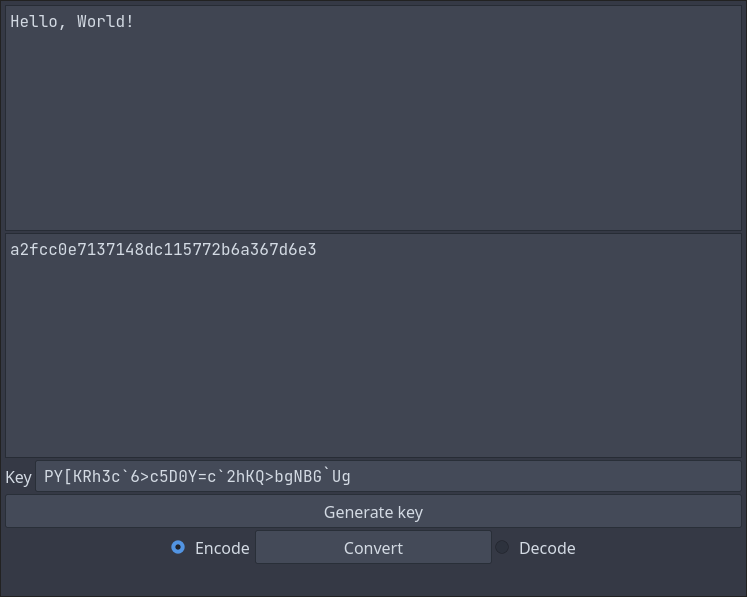
\includegraphics[width=0.8\linewidth]{figures/encode-test-1}}
    \caption{Шифрование}
\label{ris:encode-test-1}
\end{figure}

\vspace{\baselineskip}
\begin{figure}[H]
\center{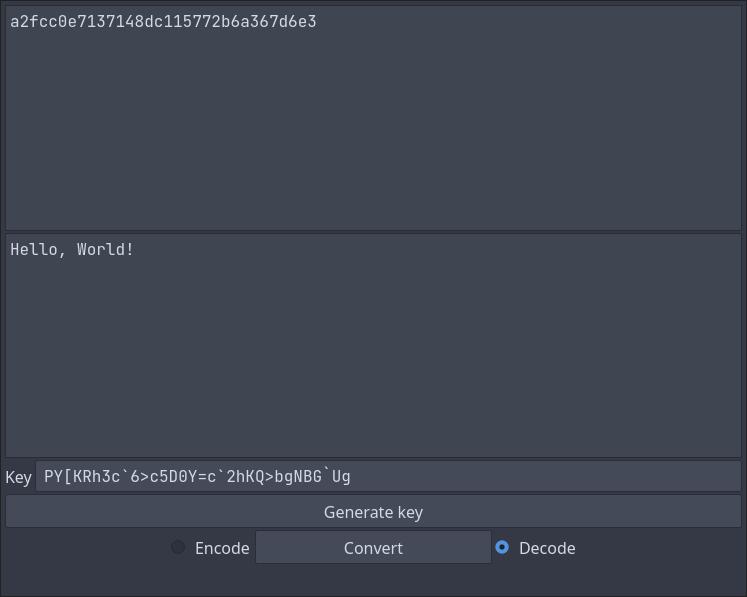
\includegraphics[width=0.8\linewidth]{figures/decode-test-1}}
    \caption{Расшифрование}
\label{ris:decode-test-1}
\end{figure}


\section{Пример 2}

\textbf{Исходный текст:} \\
    Привет, Мир! 

\textbf{Ключ:} \\
    W42JKfBHG4dU\textbackslash8G[1@?]BKJKh<]eAhIh

\textbf{Зашифрованный текст:} \\
    39e033f1ed4c218c 932c46d3e8aa4b8ff1255864c6b85fbf0cd45ea91d32386

Результаты работы программы представлены на рисунках~\ref{ris:encode-test-2}-\ref{ris:decode-test-2}.

\vspace{\baselineskip}
\begin{figure}[H]
\center{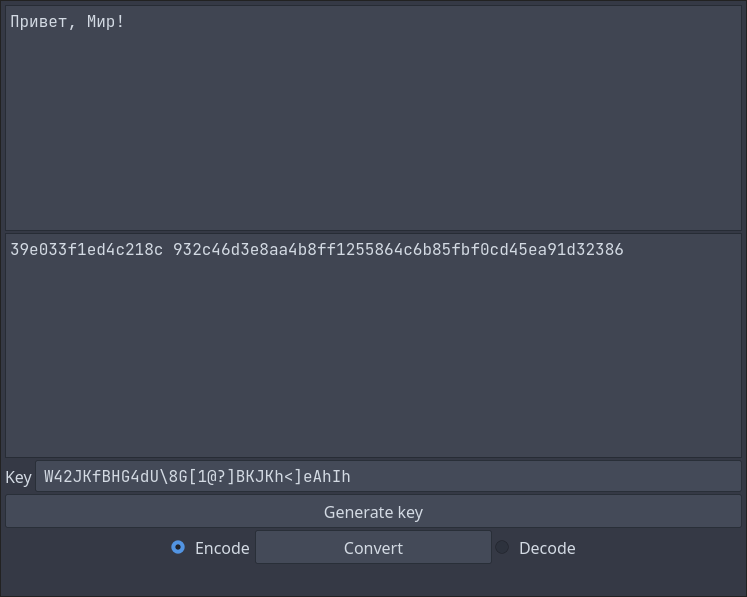
\includegraphics[width=0.8\linewidth]{figures/encode-test-2}}
    \caption{Шифрование}
\label{ris:encode-test-2}
\end{figure}

\vspace{\baselineskip}
\begin{figure}[H]
\center{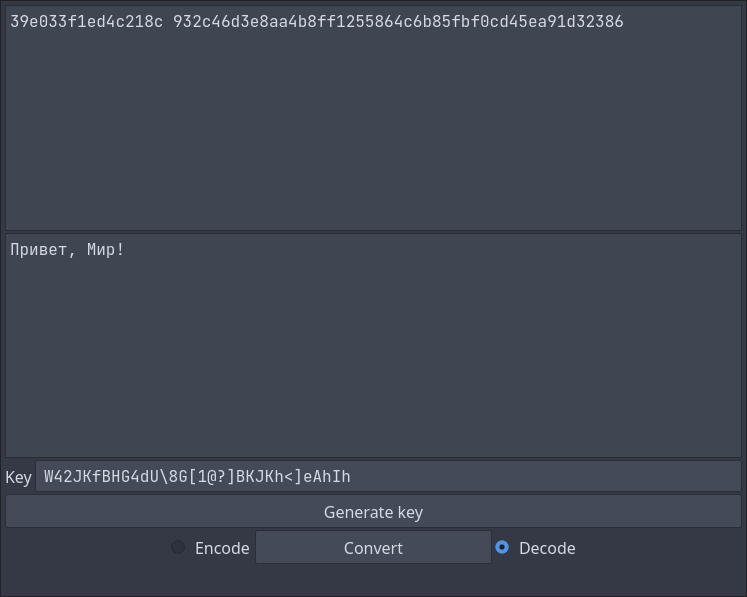
\includegraphics[width=0.8\linewidth]{figures/decode-test-2}}
    \caption{Расшифрование}
\label{ris:decode-test-2}
\end{figure}


\section{Пример 3}

\textbf{Исходный текст:} \\
    У нас есть одно критическое замечание к AES: мы не совсем доверяем
    его безопасности. Что беспокоит нас больше всего в AES, так это его
    простая алгебраическая структура… Ни один другой блочный шифр не имеет
    столь простого алгебраического представления. Мы понятия не имеем, ведёт
    это к атаке или нет, но незнание этого является достаточной причиной,
    чтобы скептически относиться к использованию AES. 

\textbf{Ключ:} \\
    ]7OAS]YO`Y;Kca`bQ`PhA99fN>NQ`WGT

\textbf{Зашифрованный текст:} \\
    aa8210d0e1b032d2e7b6c1c59428e3d5654c6e83 46d5fa898 b1744d1c4b45a469d505836303e94147795a39a15aa1394f2b110 068 fd9aace76d0e12e8fc57d84e23f7467b2df611aa794e4bea8d61246faae 0996df48b12669cd2c877fdc327ea347c 458b2 bf16078f3c3d963e4a6d11dd8661b6ada 16a1ccc2c1aee9d8a6d77d8da4047 b 0fa221ce1996d4396feb9ba8cbe26 6c3d63889d3b1b7f56e22ca7a13d5663638 3e706f68df5daf77ef277fe0f49 418b344e36ca69c1991 fc22bac14bee8368ae3 0ce7073bbcece2821abac7b e 649444113b1a45d89727ccca9aabd96c86cd0ce5dcebe953753666253dd17 4948aaed8 1222431e3274e1a80944af2d2d578a3ec93a65999ea107af62 a856549e3a0ef59695998e58df0106c482b623db d3b1a644f3169adcc759 bc5943b4665e678157acb d407b8e53aab29f1ac72bb3b2 e5d317e4c8ce2e66828866eafc62b6511f9df9984d4de45683d55b859fb 8305f29 6761962f2 66b47562957885692ac6b28b6e1c462 1dde2ca3273f24866 adfb09ff0424d3980 6ec578e504ac2c33675d16db 1106e4ff14295344b2d2c 6a8aebf79ab6d8b838 622ba26 5f177516ee11bf519145c 62cc85296d615019384a13a5d71a2 c1db1dc27a082dd42d22a 60a0467ad6 1f0d8a77335a5aa48 ecdd57aa067bf60f464cd8a5 d5e982a894dee3827a79f46c4 214fa17a785660fd31c49473d941 6e71ef8551f6 eaa6b8359d3593e183e78545d4284edb5 f4497a857cdc4 99cfae0c3 a68679c5da3caa9d6f33a4128101bec d845dea176a65d 4ef7a62cf409326354558112314175cea 4ff328875c15740a18f9e4a5e7c8293e034aae3 cab17462acfb1cabf9fad1f35022452843d 0fe7b1c311e75eeb9894f31c76d 2dc d1c2df2889c1ae7acb3a597 1e315fb c33717cb06b292464978bcd7a4b9bae 35249a31a49625e f3c8b1055a3 957f16d473cdd5b e253ebdd1ceda2ad0487b6f14e713bc e6e1c60 da6b99d b

Результаты работы программы представлены на рисунках~\ref{ris:encode-test-3}-\ref{ris:decode-test-3}.

\vspace{\baselineskip}
\begin{figure}[H]
\center{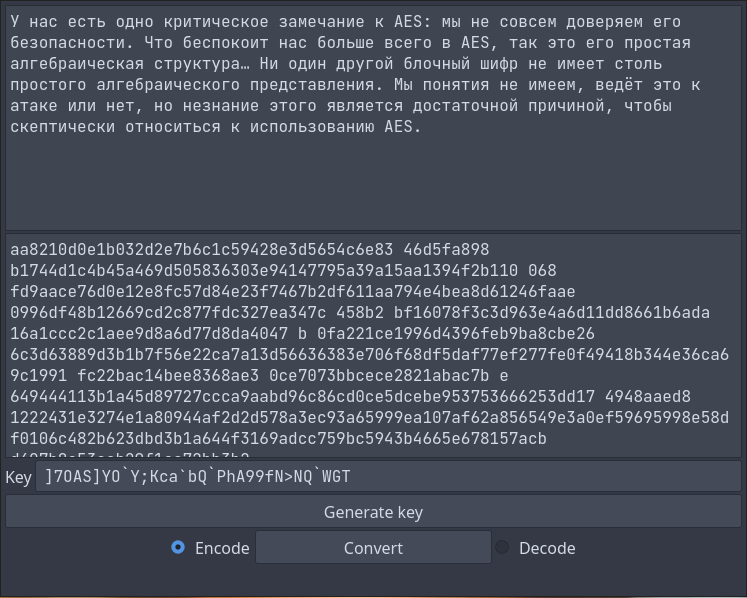
\includegraphics[width=0.8\linewidth]{figures/encode-test-3}}
    \caption{Шифрование}
\label{ris:encode-test-3}
\end{figure}

\vspace{\baselineskip}
\begin{figure}[H]
\center{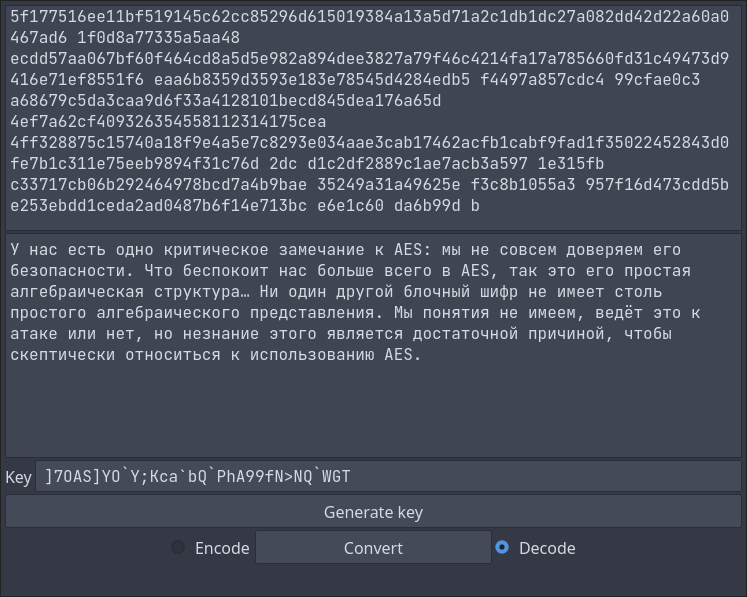
\includegraphics[width=0.8\linewidth]{figures/decode-test-3}}
    \caption{Расшифрование}
\label{ris:decode-test-3}
\end{figure}


\section{Пример 4}

\textbf{Исходный текст:} \\
    Я считаю, что в работе Куртуа-Пепшика есть ошибка. Они переоценили число
    линейно-независимых уравнений. В результате у них нет достаточного количества
    линейных уравнений для решения системы, и [указанный] метод не может взломать
    Rijndael. Он имеет определённые достоинства и заслуживает изучения, но не
    взламывает Rijndael в его нынешнем виде.

\textbf{Ключ:} \\
    3gY5c?>70b>bDNTgFF:FP3<@1S6gYQh3

\textbf{Зашифрованный текст:} \\
    3a48827e37da f48684565bde66660ed14 66fca2f2e 38fa6fbae6bc0403f495 6d83d60f67f11d2 f8aa2856edd 63a163523a298597cd895244f8962a7 74229cdb749aa3cc8a 73d6e73a5ac7de93b698087c04785fc1ad52d e7a1d44d6dc979e63386db42199e724fc2ba1c1f36c cb32e1cf1c95f2ee11f543be9139d2 539d097a32533b75e546f54 9caf980e8c3e2 9bff0ebf6 4f57c62428cb5d46b3cdd4e3765246a704d6d3c9fec65a5cdced3c1 d e208a9c858518ca46fc 1dc88b0864d9b4417e5c650909c686a4f1d4ced 361da722ab53050ffc4a5bb11 416dad0d4ea88d37074c7fc6de88ccca585c3641c f75f9ab9a9d759275f7a51cbb5b3e2f90b28e1fd03a33 d46ad14db9d db87fefaea6f0e9fbc88647af87e12b7e142 58fc8e616fca59e85fd9fa368d7ff87293d37 6d60cd24245e14e67127e272a3e975cb77fe154910284b448c32 8f2ab8558a031cf40a42851d6d7547da8dd437a6c9a8296fbc7a0 5 e4577bb 5a8871c66 c 24efbed405aa529ecf769782bee48 de6c568d4319c30722641add25c87f56c863f 12189f76889a6c5e8b9e7b611881d 056c6f547d969873343afb78172e915825042c3d1a31eea 523de862d49efd647 71bf0f112d0b8199390d675bdab7db1a883822921c71b5d35c4da9a537a24 6e83e1b4ff561163816b570936ae785abfd357be05c2e8ff09afe 1 393e02c1a904a45506a5b797426c84ca46e1f23dbb6d82f2cf674 2c3ccd4 0c56aaa7dfc9f4b63719f2c5998145b498d45561ec5a71ae13cc69bde4258def7 77af971088 abd33b2a6ca8d607342afaa 3afea7b1493f1aad34cae845c21583befd3c2 2d66960c8 5fa1ba7

Результаты работы программы представлены на рисунках~\ref{ris:encode-test-4}-\ref{ris:decode-test-4}.

\vspace{\baselineskip}
\begin{figure}[H]
\center{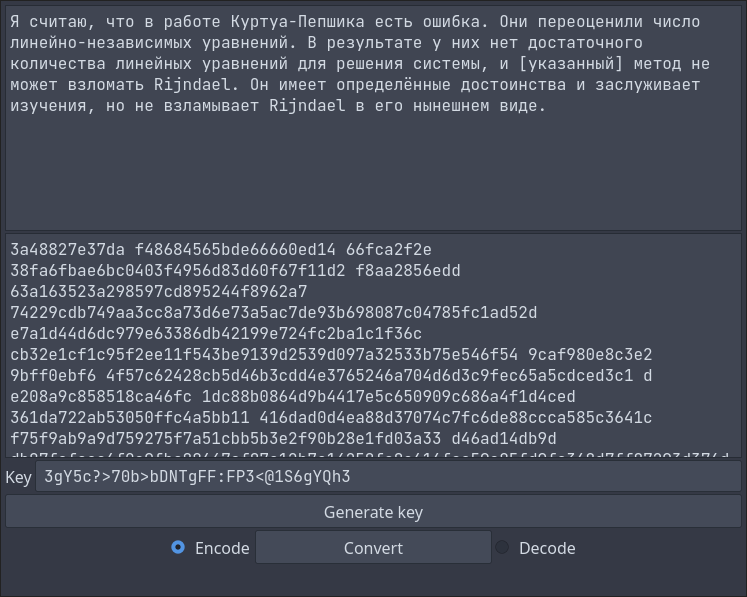
\includegraphics[width=0.8\linewidth]{figures/encode-test-4}}
    \caption{Шифрование}
\label{ris:encode-test-4}
\end{figure}

\vspace{\baselineskip}
\begin{figure}[H]
\center{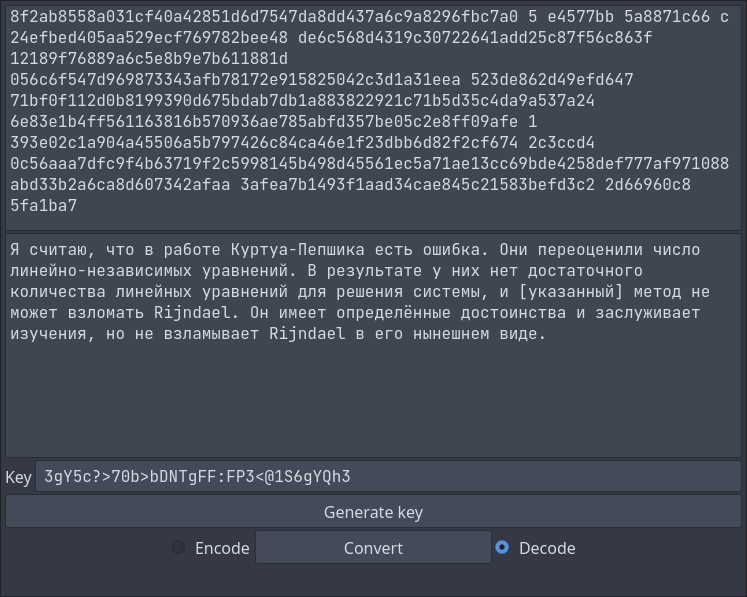
\includegraphics[width=0.8\linewidth]{figures/decode-test-4}}
    \caption{Расшифрование}
\label{ris:decode-test-4}
\end{figure}


\section{Пример 5}

\textbf{Исходный текст:} \\
    The XSL attack is not an attack. It is a dream

\textbf{Ключ:} \\
    OY8Y?Fa??FHc<4bRJ3?AFLQWFXUFPUIF

\textbf{Зашифрованный текст:} \\
    678c20e1607b836fc27446e815ac306c3c559a9bc8c6d1b5d 257f6a9893e9a6c70f36f9cb83a23123ca9b5f779c99cae

Результаты работы программы представлены на рисунках~\ref{ris:encode-test-5}-\ref{ris:decode-test-5}.

\vspace{\baselineskip}
\begin{figure}[H]
\center{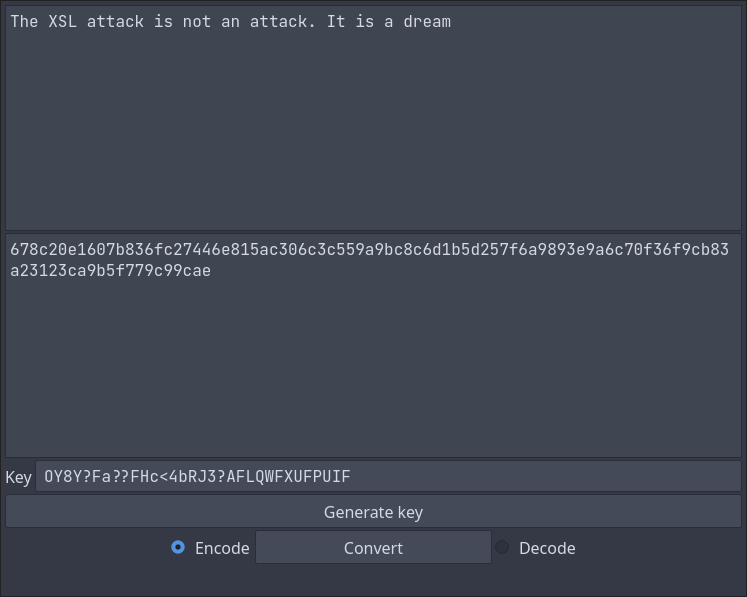
\includegraphics[width=0.8\linewidth]{figures/encode-test-5}}
    \caption{Шифрование}
\label{ris:encode-test-5}
\end{figure}

\vspace{\baselineskip}
\begin{figure}[H]
\center{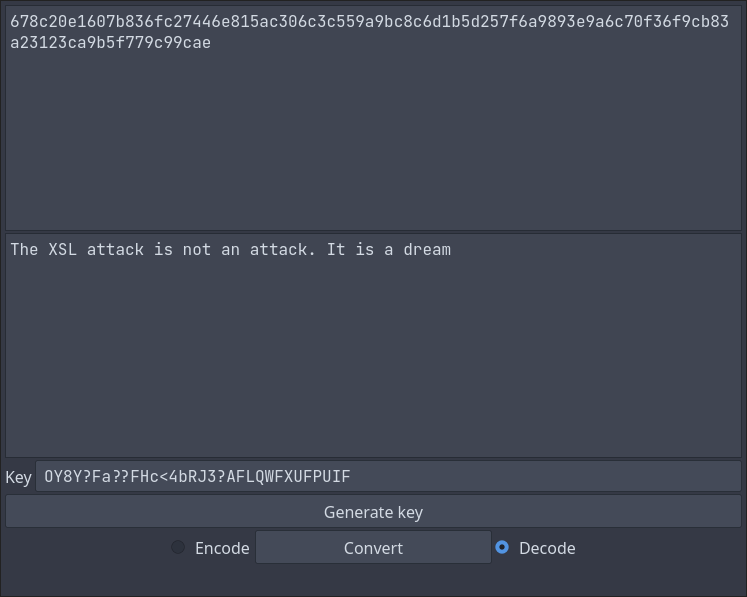
\includegraphics[width=0.8\linewidth]{figures/decode-test-5}}
    \caption{Расшифрование}
\label{ris:decode-test-5}
\end{figure}


\chapter{Исходный код}

\section{aes256.hpp}

\inputminted[fontsize=\footnotesize, breaklines]{cpp}{../../src/aes256.hpp}

\section{aes256.cpp}

\inputminted[fontsize=\footnotesize, breaklines]{cpp}{../../src/aes256.cpp}

\section{mainwindow.hpp}

\inputminted[fontsize=\footnotesize, breaklines]{cpp}{../../src/mainwindow.hpp}

\section{mainwindow.cpp}

\inputminted[fontsize=\footnotesize, breaklines]{cpp}{../../src/mainwindow.cpp}

\section{main.cpp}

\inputminted[fontsize=\footnotesize, breaklines]{cpp}{../../src/main.cpp}

\backmatter %% Здесь заканчивается нумерованная часть документа и начинаются ссылки и

\newpage
\Conclusion

В ходе работы изучил симметричный алгоритм блочного шифрования AES.

Преимущества данного алгоритма:

\begin{itemize}
\item безопасность;
\item быстродействие;
\item простота реализации.
\end{itemize}

\end{document}
